\documentclass[a4paper,sffamily,12pt]{article}

\usepackage[T1]{fontenc}
\usepackage[french]{babel}
\usepackage[utf8]{inputenc}

% Customization des listes
\usepackage{enumitem}
\usepackage{pifont}

% Insertion d'image
\usepackage{graphicx}

% Création de lien
\usepackage[colorlinks,linkcolor=blue]{hyperref}

% Formatage des titres de sections
\usepackage{titlesec}
\titleformat{\section}
  {\normalfont\Large\bfseries\sffamily}{\thesection.}{0.33em}{}[\hrule]
\titleformat{\paragraph}
  {\normalfont\bfseries\sffamily}{\theparagraph.}{0.33em}{}
 
 % tableau rectangle 
%\usepackage{slashbox}
%\usepackage{tabularx}

 % En-tête
\usepackage{fancyhdr}
\pagestyle{fancy}
\renewcommand\headrulewidth{1pt}
\fancyhead[L]{Base de données 2}
\fancyhead[R]{$X6I0050$}

% Permet de mettre du texte au dessus du titre
\usepackage{titling}
\renewcommand{\maketitlehooka}{\noindent MAHIER Loïc \hfill groupe 601B \\ JEHANNO Clément \hfill \\ JAMET Félix \hfill \\ PHALAVANDISHVILI  Demetre}

% Titre
\title{\vspace{\fill}\LARGE\bfseries\sffamily Rapport de projet\protect\footnote{rapport réalisé sous \LaTeX} \vspace{\fill}}

\begin{document}

	\date{} % Supprime la date
	\maketitle % Affiche le titre

	\thispagestyle{fancy} % Permet de mettre le titre sur la page ''fancy''
	
	\newpage
			
	\renewcommand{\contentsname}{Sommaire}
	\tableofcontents
	
	\newpage
	
	\section{Introduction}
		
		\vspace{0.5cm}
		
		Dans le cadre de ce projet nous devons créer une base de données. Nous avons décidé de modéliser la gestion de cinémas sur une grande échelle. Par exemple nous voulons savoir quels sont les cinémas de France, à qui ils appartiennent (Pathé,UGC, etc.) et ce qu'ils proposent. Comme notre modèle se base sur une certaine réalité, voici comment nous avons décomposé la chose, prenons  l'exemple d'un cinéma : \\
		\indent Le cinéma Pathé à Atlantis, dans la ville de Nantes. Tout d'abord on voit que un cinéma est identifié par une adresse et une ville. Ensuite, notre cinéma possède des salles dans lesquelles seront diffusés des films. Chaque film est composé d'une équipe d'acteurs, d'un réalisateur et d'une date de sortie. Il peut être compatible ou non avec la 3D. \\ 				
		\indent En ce qui concerne nos salles, elles possèdent un certain nombre de places qui sont réparties entre les places ''standard'', les places ''handicapés'' ainsi que les nouveaux sièges dBox (sièges bougeant en même temps que le film). Si elles sont compatibles, elles ont la possibilité de diffuser en 3D. \\
		\indent Une séance dans un cinéma donné correspond à une date de projection d'un certain film dans une salle spécifique à un horaire précis, le film étant diffusé ou non en 3D. Aujourd'hui si on va au cinéma il est possible de réserver sa séance, autrement dit, on réserve un certain nombre de places pour un film, à un horaire précis, dans un cinéma donné. 

		\vspace{0.5cm}
	
	\section{Première partie}

		\vspace{0.5cm}
								
		\subsection{Répartition des tâches}
	
			\vspace{0.5cm}
	
			\noindent Voici comment nous nous sommes organisés pour répartir les tâches : \\
			\\
			\indent Tout d'abord après les premières semaines de cours nous nous sommes réunis pour décider ensemble d'un sujet. L'idée du cinéma est venue assez naturellement et nous paraissait être à la fois concrète et proche de la réalité.\\
			\indent Ensuite nous avons défini tous les attributs de notre table, en se demandant ensemble : Que voulons-nous faire ? Comment voulons nous le faire ? Un cinéma fonctionne t-il vraiment comme ça ? L'ajout de tel ou tel attribut est-il pertinent ? etc etc. Une fois nos attributs répartis nous avons chacun pris un cinéma (on en a 4) et chaque personne a remplit la partie du tableau qui correspondait à un cinéma. Après cela on a observé nos tuples sur tableur et on a relevé nos dépendances fonctionnelles.\\
			\indent Ensuite Demetre et Félix ont fait l'algorithme de décomposition et Loïc et Clément ont fait l'algorithme de Bernstein. On a mis en commun le résultat des deux algorithmes afin de voir si on avait la même chose ou non, et pourquoi. Pour finir, nous avons testé la normalisation de notre schéma avec l'outil mis à notre disposition en question 5.
							
			\vspace{0.5cm}
			
		\subsection{Table de base}	
			
			\vspace{0.5cm}
				
			Vous trouverez en annexe la table (\ref{table_p1}) contenant tous nos attributs ainsi que tous nos tuples. Celle-ci est en quatre parties à cause de sa taille conséquente.
			
			\vspace{0.5cm}						
	
		\subsection{Dépendances fonctionnelles}
		
			\vspace{0.5cm}
		
			A partir de la table ci-dessous contenant tous nos attributs, nous avons déduit les douze dépendances fonctionnelles ci-dessous. Pour ce faire nous avons ajouté des attributs (id) nous permettant de simplifier nos relations.\\
		
			\noindent- (1) idCine $\rightarrow$ adresse, ville \\
			- (2) adresse, ville $\rightarrow$ franchise, nbSalle \\
			- (3) idCine $\rightarrow$ franchise, nbSalles \\
			- (4) idCine, numSalle $\rightarrow$ salleCompatibleEn3D, nbPlaceStandard, nbPlaceHandicape,nbDbox \\
	 		- (5) idFilm $\rightarrow$ nomFilm, dateSortie \\
			- (6) nomFilm, dateSortie $\rightarrow$ public, idReal, duree, compatible3D \\
			- (7) idFilm, role $\rightarrow$  idAct \\
			- (8) idReal $\rightarrow$ nomR, prenomR \\
			- (9) idAct $\rightarrow$ nomA, prenomA \\
			- (10) idClient $\rightarrow$ nomC, prenomC \\
			- (11) idClient, numReservation $\rightarrow$ nbPlaceStandardRes, nbPlaceHandicapeRes, nbPlaceDBoxRes, idSeance \\
			- (12) idSeance $\rightarrow$ idCine, horaire, dateProjection, numSalle, idFilm, diffusionEn3D \\
			
			\newpage
			
			Avec les dépendances fonctionnelles ci-dessus, nous obtenons le graphe des dépendances en annexe (\ref{graphe_dependances}). De cela nous déterminons la clé suivante : \{idCine, idClient, numReservation, role\}.
			
		\subsection{Algorithme de Bernstein}
		
			\vspace{0.5cm}
	
			\noindent L'algo de Bernstein se fait en 4 parties :
		
				\begin{enumerate}[label=\ding{228}]
					\item Calculer la CV(DF) et les clés. Si R est en 3FN on s'arrête. 
					\item Partitionner CV(DF) en groupe DFi (1 <= i <= k) tel que toutes les dfs d'un même groupe aient la même partie gauche. 
					\item Construire un schéma <Ri(Ui), DFi> pour chaque groupe DFi, où Ui est l'ensemble des attributs apparaissant dans DFi.
					\item Si aucun des schémas définis ne contient de clé X de R, rajouter un schéma <Rk+1(X), \{\}>.
				\end{enumerate}	
				
			\subsubsection{Calcul de CV(DF)}
	
				\vspace{0.5cm}
	
				\noindent La couverture minimale se fait en trois parties :
	
				\begin{enumerate}[label=\ding{228}]
					\item Toutes les dépendances doivent être élémentaires ; les décomposer si nécessaire.
					\item Eliminer les attributs superflus du coté gauche de la df.
					\item Eliminer les dfs redondantes.
				\end{enumerate}	
				
				\vspace{0.5cm}
					
				\paragraph{Pas 1}
	
					\vspace{0.5cm}
	
					\noindent On décompose chacune des dfs en dfe : \\
	
					\noindent- (1) idCine $\rightarrow$ ville \\
					- (1) idCine $\rightarrow$ adresse \\
					- (2) adresse, ville $\rightarrow$ franchise \\
					- (2) adresse, ville $\rightarrow$ nbSalle \\
					- (3) idCine $\rightarrow$ franchise \\
					- (3) idCine $\rightarrow$ nbSalles \\
					- (4) idCine, numSalle $\rightarrow$ salleCompatibleEn3D \\
			 		- (4) idCine, numSalle $\rightarrow$ nbPlaceStandard \\
			 		- (4) idCine, numSalle $\rightarrow$ nbPlaceHandicape \\
			 		- (4) idCine, numSalle $\rightarrow$ nbDbox \\
			 		- (5) idFilm $\rightarrow$ nomFilm \\
			 		- (5) idFilm $\rightarrow$ dateSortie \\				 		
					- (6) nomFilm, dateSortie $\rightarrow$ public \\
					- (6) nomFilm, dateSortie $\rightarrow$ idReal \\
					- (6) nomFilm, dateSortie $\rightarrow$ duree \\
					- (6) nomFilm, dateSortie $\rightarrow$ compatible3D \\
					- (7) idFilm, role $\rightarrow$ idAct \\
					- (8) idReal $\rightarrow$ nomR \\
					- (8) idReal $\rightarrow$ prenomR \\						
					- (9) idAct $\rightarrow$ nomA \\
					- (9) idAct $\rightarrow$ prenomA \\						
					- (10) idClient $\rightarrow$ nomC \\
					- (10) idClient $\rightarrow$ prenomC \\						
					- (11) idClient, numReservation $\rightarrow$ idSeance \\
					- (11) idClient, numReservation $\rightarrow$ nbPlaceStandardRes \\
					- (11) idClient, numReservation $\rightarrow$ nbPlaceHandicapeRes \\
					- (11) idClient, numReservation $\rightarrow$ nbPlaceDBoxRes \\
					- (12) idSeance, idCine $\rightarrow$ horaire \\
					- (12) idSeance, idCine $\rightarrow$ dateProjection \\
					- (12) idSeance, idCine $\rightarrow$ numSalle \\
					- (12) idSeance, idCine $\rightarrow$ idFilm \\
					- (12) idSeance  idCine $\rightarrow$ diffusionEn3D \\
			
					\vspace{0.5cm}
										
				\paragraph{Pas 2}
	
					\vspace{0.5cm}
		
					On prend toutes les dfs qui ont plus d'un attribut à gauche et on calcul leur fermeture. On élimine l'autre attribut si l'attribut de droite de la df apparaît dans le résultat, ou s'il apparaît dans le résultat de la fermeture. \\
					
					\noindent - (2) adresse, ville $\rightarrow$ franchise, nbSalle \\
						\\
						\underline{adresse+} \\
						adresse \\
						\underline{ville+} \\
						ville \\
					$\rightarrow$ Les deux attributs sont nécessaires. \\
	
					\noindent - (4) idCine, numSalle $\rightarrow$ salleCompatibleEn3D, nbPlaceStandard, nbPlaceHandicape,nbDbox \\
						\\
						\underline{idCine+} \\
						idCine / adresse / ville /franchise / nbSalle \\
						\underline{numSalle+} \\
						numSalle \\
					$\rightarrow$ Les deux attributs sont nécessaires. \\
					
					\noindent - (6) nomFilm, dateSortie $\rightarrow$ public, idReal, duree, compatible3D \\																						\\
						\underline{nomFilm+} \\
						nomFilm \\
						\underline{dateSortie+} \\
						dateSortie \\
					$\rightarrow$ Les deux attributs sont nécessaires. \\
				
					\noindent - (7) idFilm, role $\rightarrow$  idAct \\
						\\
						\underline{idFilm+} \\
						idFilm / nomFilm / dateSortie / public / idReal / duree / compatible3D / nomA / prenomA \\
						\underline{role+} \\
						role \\
					$\rightarrow$ Les deux attributs sont nécessaires. \\
						
					\noindent - (11) idClient, numReservation $\rightarrow$ nbPlaceStandardRes, nbPlaceHandicapeRes, nbPlaceDBoxRes, idSeance \\
						\\
						\underline{idClient+} \\
						idClient / nomC / prenomC \\
						\underline{numReservation+} \\
						numReservation \\	
					$\rightarrow$ Les deux attributs sont nécessaires. \\					
					
					\noindent - (12) idSeance, idCine $\rightarrow$ horaire, dateProjection, numSalle, idFilm, diffusionEn3D \\												
						\\
						\underline{idSeance+}\\
						idSeance \\
						\underline{idCine+}
						adresse / ville / franchise / nbSalle \\
					$\rightarrow$ Les deux attributs sont nécessaires. \\
	
					\vspace{0.5cm}
	
				\paragraph{Pas 3}		
		
					\vspace{0.5cm}
		
					\noindent Eliminons tout d'abord les dfs qui sont préservées par transitivité : \\
		
						\noindent- (1) idCine $\rightarrow$ adresse, ville \\
						- (2) adresse, ville $\rightarrow$ franchise, nbSalle \\
						- (3) idCine $\rightarrow$ franchise, nbSalles \\
						
					Si l'on prend les dfs 1, 2 et 3, on remarque que l'on peut supprimer la 3 car on peut retrouver celle-ci par transitivité. Reprenons donc nos dfs restantes : \\
						
					\noindent- (1) idCine $\rightarrow$ adresse, ville \\
					- (2) adresse, ville $\rightarrow$ franchise, nbSalle \\
					- (3) idCine, numSalle $\rightarrow$ salleCompatibleEn3D, nbPlaceStandard, nbPlaceHandicape,nbDbox \\
			 		- (4) idFilm $\rightarrow$ nomFilm, dateSortie \\
					- (5) nomFilm, dateSortie $\rightarrow$ public, idReal, duree, compatible3D \\
					- (6) idFilm, role $\rightarrow$  idAct \\
					- (7) idReal $\rightarrow$ nomR, prenomR \\
					- (8) idAct $\rightarrow$ nomA, prenomA \\
					- (9) idClient $\rightarrow$ nomC, prenomC \\
					- (10) idClient, numReservation $\rightarrow$ nbPlaceStandardRes, nbPlaceHandicapeRes, nbPlaceDBoxRes, idSeance \\
					- (11) idSeance, idCine $\rightarrow$ horaire, dateProjection, numSalle, idFilm, diffusionEn3D \\
					
					\noindent A présent, analysons chaque dépendance fonctionelle une par une : \\
					
					\noindent - (1) idCine $\rightarrow$ adresse, ville \\
						\\
						\underline{idCine+} \\
						idCine\\									
					$\rightarrow$ La df est préservée. \\		
						
					\noindent - (2) adresse, ville $\rightarrow$ franchise, nbSalle \\
						\\
						\underline{adresse, ville+} \\
						adresse, ville \\									
					$\rightarrow$ La df est préservée. \\
					
					\noindent - (3) idCine, numSalle $\rightarrow$ salleCompatibleEn3D, nbPlaceStandard, nbPlaceHandicape,nbDbox \\
						\\
						\underline{idCine, numSalle+} \\
						idCine / adresse / ville / franchise / nbSalle / numSalle \\								
					$\rightarrow$ La df est préservée. \\													
	
					\noindent - (4) idFilm $\rightarrow$ nomFilm, dateSortie \\
						\\
						\underline{idFilm+} \\
						idFilm\\								
					$\rightarrow$ La df est préservée. \\	
					
					\noindent - (5) nomFilm, dateSortie $\rightarrow$ public, idReal, duree, compatible3D \\
						\\
						\underline{nomFilm, dateSortie+} \\
						nomFilm / dateSortie \\									
					$\rightarrow$ La df est préservée. \\	
					
					\noindent - (6) idFilm, role $\rightarrow$  idAct  \\
						\\
						\underline{idFilm, role+} \\
						idFilm / nomFilm / dateSortie / public / idReal / duree / compatible3D / nomR / prenomR / role \\					
					$\rightarrow$ La df est préservée. \\
																				
					\noindent - (7) idReal $\rightarrow$ nomP, prenomP \\
						\\
						\underline{idReal+} \\
						idReal \\								
					$\rightarrow$ La df est préservée. \\	
					
					\noindent - (8) idAct $\rightarrow$ nomP, prenomP \\
						\\
						\underline{idAct+} \\
						idAct \\									
					$\rightarrow$ La df est préservée. \\	
	
					\noindent - (9) idClient $\rightarrow$ nomC, prenomC \\
						\\
						\underline{idClient+} \\
						idClient \\									
					$\rightarrow$ La df est préservée. \\		
	
					\noindent - (10) idClient, numReservation $\rightarrow$ nbPlaceStandardRes, nbPlaceHandicapeRes, nbPlaceDBoxRes, idSeance \\
						\\
						\underline{idClient, numReservation+} \\
						idClient / nomC / prenomC / numReservation \\									
					$\rightarrow$ La df est préservée. \\		
	
					\noindent - (11) idSeance, idCine $\rightarrow$ horaire, dateProjection, numSalle, idFilm, diffusionEn3D \\
						\\
						\underline{idSeance, idCine+} \\
						idSeance / idCine / adresse / ville / franchise / nbSalle \\							
					$\rightarrow$ La df est préservée. \\							
					\\		
					
					\indent Ainsi, hormis la suppression d'une dépendance fonctionnelle transitive, nos dépendances fonctionelles ne changent pas. \\																
					\\
					\indent On constate que l'on est bien en 1FN, ainsi qu'en 2FN. Cependant nous ne sommes pas en 3FN. En effet, nous avons des attributs non clés, qui déterminent d'autres attributs non clés. Par exemple, adresse et ville sont deux attributs non clés qui déterminent franchise et nbSalle qui sont eux aussi non clés (df(2)). \\
					
					\vspace{0.5cm}
														
				\subsubsection{Partitionnement de la CV et construction des schémas} 	
				
					\vspace{0.5cm}
				
					\noindent R1 = \{\underline{idCine}, adresse, ville\} \\  DF1 = \{idCine $\rightarrow$ adresse, ville\} \\
					\\
					R2 = \{\underline{adresse, ville}, franchise, nbSalle\} \\ DF2 = \{adresse, ville $\rightarrow$ franchise, nbSalle\} \\
					\\
					R3 = \{\underline{idCine, numSalle}, salleCompatibleEn3D, nbPlaceStandard, nbPlaceHandicape, nbDbox\} \\ DF3 = \{idCine, numSalle, $\rightarrow$ salleCompatibleEn3D, nbPlaceStandard, nbPlaceHandicape, nbDbox\} \\
					\\
					R4 = \{\underline{idFilm}, nomFilm, dateSortie\} \\ DF4 = \{idFilm $\rightarrow$ nomFilm, dateSortie\} \\
					\\
					R5 = \{\underline{nomFilm, dateSortie}, public, idReal, duree, compatible3D\} \\ DF5 = \{nomFilm, dateSortie $\rightarrow$ public, idReal, duree, compatible3D\} \\	
					\\							
					R6 = \{\underline{idFilm, role}, idAct\} \\ DF6 = \{idFilm, role $\rightarrow$  idAct\} \\
					\\
					R7 = \{\underline{idReal}, nomR, prenomR\} \\ DF7 = \{idReal $\rightarrow$ nomR, prenomR\} \\
					\\
					R8 = \{\underline{idAct}, nomA, prenomA\} \\ DF8 = \{idAct $\rightarrow$ nomA, prenomA\} \\
					\\
					R9 = \{\underline{idClient}, nomC, prenomC\} \\ DF9 = \{idClient $\rightarrow$ nomC, prenomC\} \\ 
					\\
					R10 = \{\underline{idClient, numReservation}, nbPlaceStandardRes, nbPlaceHandicapeRes, nbPlaceDBoxRes, idSeance\} \\ DF10 = \{idClient, numReservation $\rightarrow$  nbPlaceStandardRes, nbPlaceHandicapeRes, nbPlaceDBoxRes, idSeance\} \\
					
					\newpage 
					
					R11 = \{\underline{idSeance, idCine}, horaire, dateProjection, numSalle, idFilm, diffusionEn3D\} \\ DF11 = \{idSeance, idCine $\rightarrow$ horaire, dateProjection, numSalle, idFilm, diffusionEn3D\} \\
					
					On constate que nous n'avons pas de relation contenant toutes nos clés, c'est pourquoi nous devons créer une relation pour cela, avec une dépendance fonctionnelle associée vide.\\
												
					\noindent R12 = \{\underline{idCine, idClient, numReservation, role}\} \\ DF12 = \{\} \\
	
					\vspace{0.5cm}
	
			\subsection{Algorithme de décomposition}
	
				\vspace{0.5cm}
				
				Nous avons pris tous nos attributs puis nous avons suivi l'algorithme de décomposition. C'est à dire que en fonction de nos attributs et de nos dépendances fonctionnelles, nous avons pris une dépendance et avons fait une relation en fonction de cette dépendance. Puis nous avons retiré nos attributs non clés du reste de la relation originale. Ensuite on a recommencé jusqu'à arriver à une partie ne contenant que des clés et plus de dépendance fonctionnelle.\\
				\indent On a commencé par les dépendances fonctionelles qui n'avaient qu'un attribut à gauche puis nous avons fini par celles qui avaient plusieurs attributs à gauche.
	
			\newpage
			
					\begin{figure}[!h]		
						\hspace{-2cm}
						{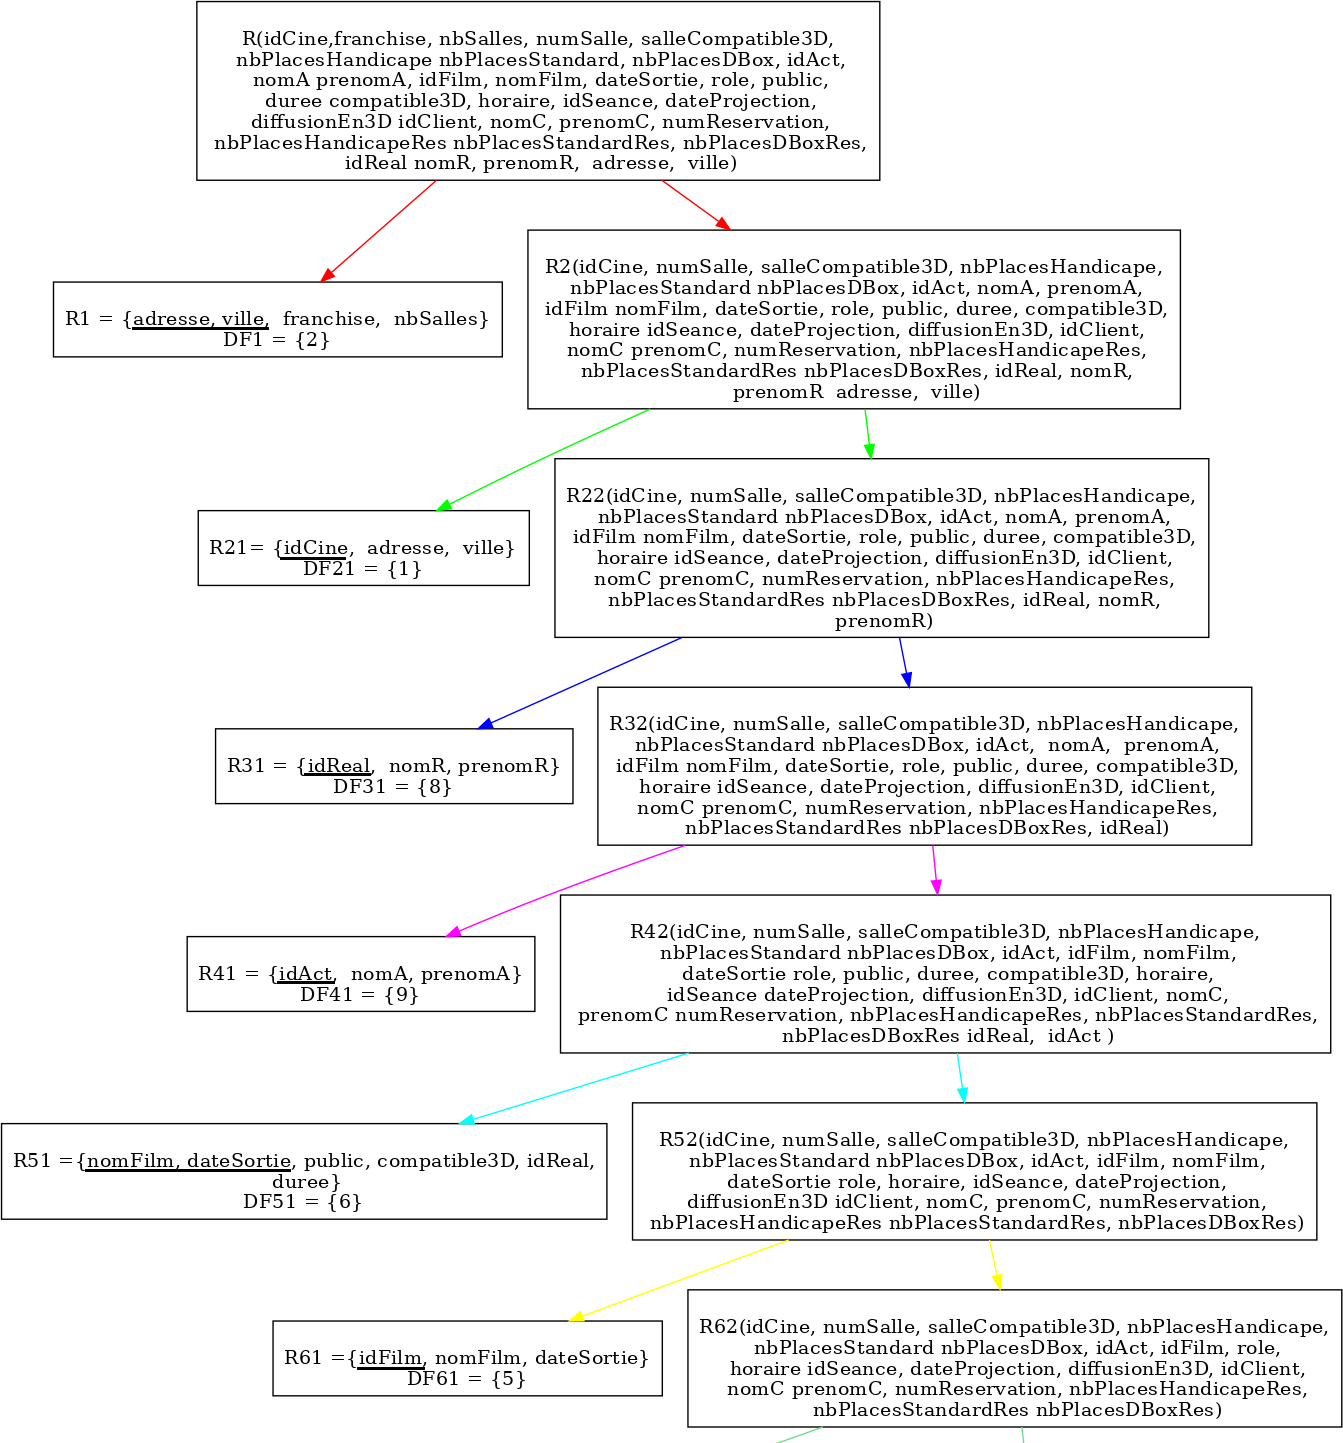
\includegraphics[height=19cm]{picture/decomp1.png}}
						\caption{Première partie de notre algorithme de décomposition}
						\label{decomp1}	
					\end{figure}	
				
					\begin{figure}[!h]		
						\hspace{-2cm}
						{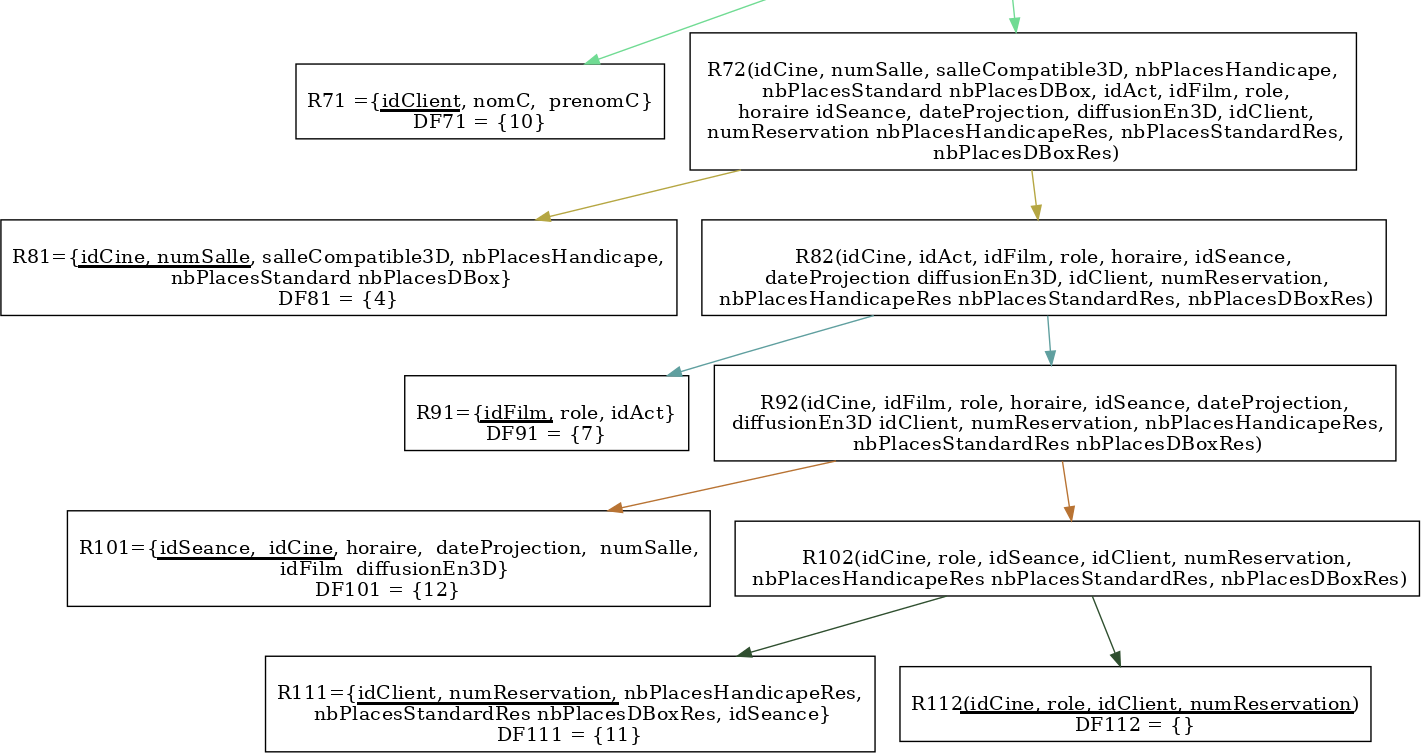
\includegraphics[height=9cm]{picture/decomp2.png}}
						\caption{Deuxième partie de notre algorithme de décomposition}
						\label{decomp2}	
					\end{figure}		
	
				\vspace{0.5cm}
			
			\subsection{Schéma de nos tables}
	
				\vspace{0.5cm}
						
			Pour le diagramme nous nous sommes basés sur le résultat de l'algorithme de décomposition qui nous a fourni des tables équivalentes aux 11 relations R1..R11. Cependant nous avons fusionné deux fois deux tables : la table R1 et R21 car cela nous paraît plus logique d'avoir pour chaque adresse, ville, franchise et nbSalles un seul idCine qui détermine un unique cinéma.\\
			\indent Cette table devient donc la table Cinema, ce qui donne plus de sens à notre modèle. Nous avons aussi fusionné R51 et R61 pour en faire une seule et même table Film pour les mêmes raisons.\\
			\indent Pour finir on a renommé toutes les autres tables pour leur donner un nom plus parlant : R31 est devenue Realisateur, R41 est devenue Acteur, R71 est devenue Client, R81 est devenue Salle, R91 est devenue Casting, R101 est devenue Seance et 111 est devenue Reservation.
	
					\begin{figure}[!h]		
						\hspace{-0.5cm}
						{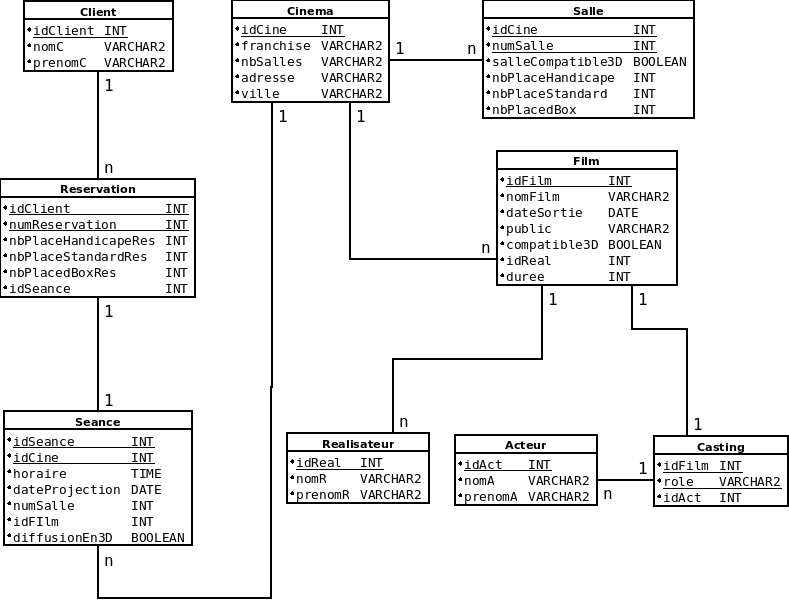
\includegraphics[height=12cm]{picture/DiagrammeUML.png}}
						\caption{Diagramme UML de nos tables}
						\label{UML}
						\vspace{0.5cm}	
					\end{figure}		
	
	
			\newpage
	
			\subsection{Conclusion préliminaire}
	
				\vspace{0.5cm}
				
				Cette première partie nous a permis de bien poser les bases de notre base de donnée. De plus, l'algorithme de décomposition nous permet d'obtenir des tables qui nous semblent cohérentes avec la réalité. Pour la suite, nous avons déjà quelques idées de contraintes, de triggers et de fonctions qu'il nous faudra intégrer pour bien gérer nos cinémas. \\			

			\newpage

	\section{Deuxième partie}

		\vspace{0.5cm}

		\subsection{Modifications de nos schémas}			

				\vspace{0.5cm}

				Suite au dépôt de la première partie du projet concernant principalement nos tables, nous avons remarqué quelques incohérences. Nous allons commencer cette deuxième partie du rapport par corriger ces défauts, ainsi nous pourrons continuer sur une base saine. Tout d'abord, avec le schéma précédemment obtenu, un film ne pouvait avoir plusieurs rôles, ce qui est incorrect. Nous avons donc rectifiés la cardinalité entre les tables Casting et Film. D'autre part, nous avions un problème similaire entre les tables Séance et Réservation. En effet on ne pouvait avoir qu'une réservation par séance. 
				\indent Ensuite, et c'est peut-être le problème majeur, nous avions une incohérence au niveau de nos clés primaires pour la table Séance, ce qui bloquait la jointure naturel entre Séance et Réservation. Comme idCine était clé primaire dans Séance, il aurait fallu ajouter dans Réservation la clé idCine pour pouvoir faire une jointure naturel. Cependant, nous avons préféré enlever idCine de la clé primaire de la table Réservation, pour la raison que nous ne voulons pas qu'une réservation soit propre au cinéma, mais globale. 
				\indent Enfin, en réfléchissant sur le type de variable de l'attribut horaire, on s'est rendu compte que le type "TIME" était obsolète. Ainsi, au lieu d'avoir deux variables dateProjection et horaire, nous avons décidé d'avoir une seule variable qui contient à la fois la date et l'heure de la projection. Aussi nous avons toujours la possibilité de faire des comparaisons car ce format de date nous le permet. \\
				
				Voici le nouveau diagramme UML : \\

				\newpage
				
					\begin{figure}[!h]		
						\hspace{-1cm}
						{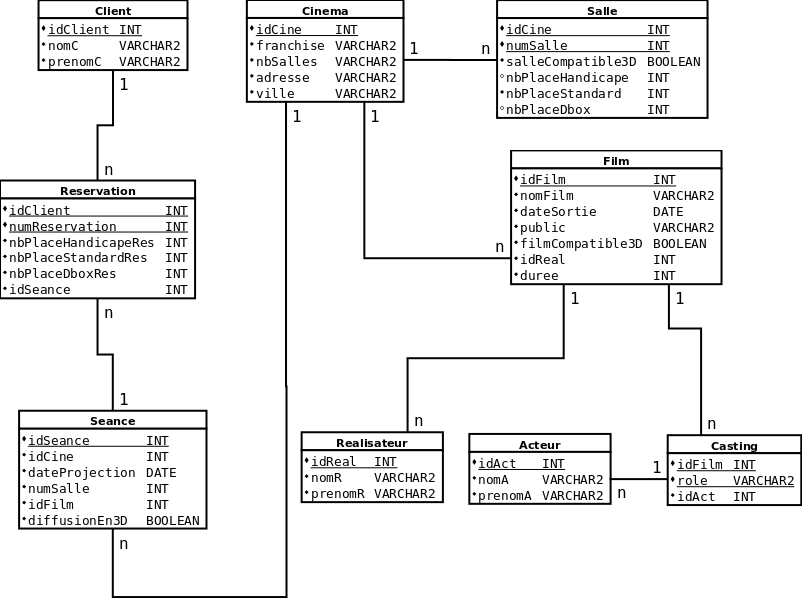
\includegraphics[height=12cm]{picture/DiagrammeUML_corrige.png}}
						\caption{Nouveau diagramme UML de nos tables}
						\label{UML}
						\vspace{0.5cm}	
					\end{figure}
		
				\vspace{0.5cm}
					
		\subsection{Répartition des tâches}

				\vspace{0.5cm}

				Au début, nous nous sommes réunis tous les quatre pour discuter des problèmes qui se posaient suite à la première partie et apporter les modifications nécessaires (voir ci-dessus). Ensuite, on s'est répartis les tâches comme suit : Demetre a travaillé sur les triggers, Loïc a fait les vues et une procédure à l'aide de Clément et enfin, Félix a fait les insertions de tuples ainsi qu'une procédure. Pour finir, Loïc et Clément ont rédigés le rapport pendant que Demetre et Félix faisaient les jeux d'essais.


		\subsection{Explications}

				\vspace{0.5cm}

				\subsubsection{Les triggers}
				
					\vspace{0.5cm}

					\begin{enumerate}[label=\ding{228}]
					
						\item verif3D : \\
						
							Le trigger verif3D a pour rôle de s'assurer qu'une séance diffusée en 3D est projetée dans une salle compatible avec la projection en 3D. Une exception est levée si la séance est en 3D mais que la salle n'est pas compatible 3D. Ainsi, une salle compatible 3D peut parfaitement projeter des films non 3D.\\
											
						\item verifPlace: \\
						
							Avant d'insérer ou de faire une modification sur Reservation on vérifie qu'on excède pas la capacité de la salle. On va donc calculer toutes les places qui sont réservées, on additionne le nombre de places déjà réservées avec le nombre de places qu'on veut réserver et si on excède la capacité de la salle alors on lève une exception suivant le nombre de place qui pose problème. En effet, on distingue chaque type de place, une personne peut réserver 10 places standard et 1 place dbox, si il y a 0 place dbox mais 50 places standard il faut lui dire qu'il n'y a pas assez de places dbox mais assez de places standard.\\
						
					\end{enumerate}

				\subsubsection{Les vues}
				
					\vspace{0.5cm}

					\begin{enumerate}[label=\ding{228}]

						\item seanceDisponible: \\
						
							Cette vue a été pensée pour le client, en effet elle indique les séances disponibles à partir de la date du système pour lesquelles il reste encore des places à réserver. Ainsi elle retourne le titre du film, la date de projection, le nom du cinéma et la salle. \\
												
						\item seanceAVenir : \\
						
						Cette vue nous permet de faire un zoom sur les séances qui n'ont pas encore eu lieu. On récupère donc tout sur la table Seance avec pour condition d'avoir une date ultérieure à la date actuelle. Cette vue nous a été utile dans le cadre d'une fonction de réservation.\\
																	
					\end{enumerate}					
								
				\subsubsection{Les procédures}
				
					\vspace{0.5cm}

					\begin{enumerate}[label=\ding{228}]

						\item reservationClient: \\
						
							La procédure reservationClient prend en paramètre un nom, un prénom et une séance ainsi que le nombre de places qu'on veut réserver. Comme quand on va au cinéma, si on veut réserver on précise combien de places on prend. Le nom et le prénom nous servent à savoir si le Client est déjà dans la base ou non. On a donc deux tests : déjà on veut savoir si on peut réserver c'est ici qu'on se sert de notre vue : on regarde si la séance est bien à venir et qu'elle n'est pas déjà passée. Une fois que c'est fait on regarde si le client est dans la base : si il l'est, on récupère son id et on ajoute directement sa réservation, sinon on l'ajoute dans la base des clients et on fait ensuite sa réservation avec le nouvel identifiant que l'on vient de lui attribuer.\\
												
						\item affichPlaces : \\
						
							Cette fonction prend en paramètre l'identifiant d'une séance et affiche le nombre de places standard, handicapé et dbox restantes. Elle pourrait être utile à un guichetier voulant s'assurer que les places qu'il s'apprête à vendre sont disponibles. Dans un premier temps, cette fonction calcule pour chaque type de place : le nombre ayant été réservé pour la séance fournie en paramètre et le nombre de places dans la salle dans laquelle la séance a lieu (la capacité de la salle). Le nombre de places restante est la capacité de la salle à laquelle on soustrait le nombre de places réservées.\\
																	
					\end{enumerate}

					\newpage

				\subsubsection{Les droits}
				
					\vspace{0.5cm}
					
					Avant toute chose, on se place dans un contexte d'utilisation externe de la base de données, par exemple dans le cas où nous arrivons à un cinéma et nous pouvons donc consulter une programmation ou traiter avec des guichetiers. \\ 

					\begin{enumerate}[label=\ding{228}]

						\item lesClients : \\
						
							On simule ici les droits que possède un client, ou plus simplement un utilisateur du site web. Le client aura seulement les droits de lecture sur la table ainsi il pourra rechercher le titre d'un film ou bien même un cinéma. Ils ont donc un accès en lecture sur les tables Seance, Cinema et Film.\\
																		
						\item lesGuichetiers : \\
						
							Nos guichetiers sont ceux qui vont réserver les places ils ont donc un accès en lecture sur les tables Seance et Reservation. Ainsi qu'un accès en écriture sur la table Reservation. Cependant, il doit vérifier si le client est dans la base donc on lui permet aussi un droit de sélection sur la table Client, si il n'y est pas il peut l'ajouter donc on lui donne un droit d'écriture.\\
						
						\item lesGerantsFilm : \\
							
							Les gérants des films et donc de la programmation vont agencer les films et les séances pour le cinéma. Ils ont un droit de lecture sur les films et les salles mais aussi de modification sur les séances. Ainsi ils peuvent créer leurs séances pour gérer leur cinéma.\\
																													
					\end{enumerate}
					
				\subsubsection{Les index}
				
					\vspace{0.5cm}
					
					Les clés primaires étant déjà indexées par défaut, nous avons rajouté deux index d'attributs non primaires qui nous semblaient utiles. Cette fois ci, on se place dans le cas d'un client qui fait une recherche sur internet. \\ 					
					
					\begin{enumerate}[label=\ding{228}]

						\item nomFilm : \\
						
							La plupart des clients savent quel film ils vont voir, ils cherchent donc à savoir où et quand est diffusé ce film. Ceci est un exemple pour montrer que l'attribut titre est un attribut qui sera beaucoup sollicité, son indexation permettra donc de gagner du temps sur nos requêtes et donc que la recherche du client soit plus rapide.\\
																		
						\item ville : \\
						
							De même, il nous semble pertinent de savoir quels cinémas se trouvent dans notre ville. \\					
																													
					\end{enumerate}
										
		\subsection{Atouts, améliorations envisageables et critique}
				
			\vspace{0.5cm}
			
				Commençons par les atouts : notre base de données repose sur une idée concrète et proche de la réalité. On a essayé de se placer dans la peau des divers personnages qui peuvent avoir rapport de près ou de loin à notre base de données (client, gérant, guichetier, etc.). Grâce à la manière dont nos tables sont faites et à nos index, les requêtes qui sont les plus évidentes (rechercher un film, un cinéma, trouver une séance, etc.) sont des requêtes qui seront assez rapides car elles viennent chercher sur nos attributs clés ou bien nos attributs indexés.\\
				\indent Nous avons quelques idées d'améliorations, par exemple nous pourrions rajouter des fonctionnalités qui permettent au client de réserver lui-même une séance (ainsi, pas besoin de passer par un guichetier, c'est le cas dans le cadre d'un webservice). Aussi, toujours dans le but de rendre notre base de données le plus proche possible de la réalité chaque film pourrait avoir un synopsis. Une table Avis pourrait être rajoutée contenant pour chaque client un commentaire et une note sur un film. Plus généralement on pourrait aussi ajouter des notions de prix pour les séances (modulable suivant la 3D et le cinéma).\\
				\indent Les points noirs de notre projet sont essentiellement au niveau de la cohérence de la base, on a pas toujours été le plus cohérent possible avec la réalité car on avait du mal à trouver un compromis entre réalité et gestion de base de données. \\
				
														
	\section{Conclusion}

		\vspace{0.5cm}
				
			Le projet de base de données nous a permis d'acquérir des notions de sqlplus et d'approfondir ce que nous avions déjà vu en L1. Nous avons eu du mal à bien définir notre projet et à savoir si nous pensions bien la chose, ce qui a été assez formateur pour se rendre compte de nos erreurs et des mauvais choix. Par exemple, entre le premier rapport et celui-ci nous avons changé de point de vue sur la base. Cela nous a aussi permis de mieux comprendre l'objectif d'une base de données vis à vis d'une application concrète en se demandant "que peut faire un client", "comment on pourrait voir ça depuis un site web", "comment la personne qui gère les films peut agencer ses séances", etc.\\
			\indent La base de données est donc un outil très utile en pratique et c'est grâce à ce genre de projets qu'on réalise que absolument toutes les applications concrètes en nécessitent (gestion de stocks, de personnel, etc.\\

		\newpage
	
	\section{Annexe}
					
		\begin{figure}[!h]		
			\centering
			\rotatebox{90}{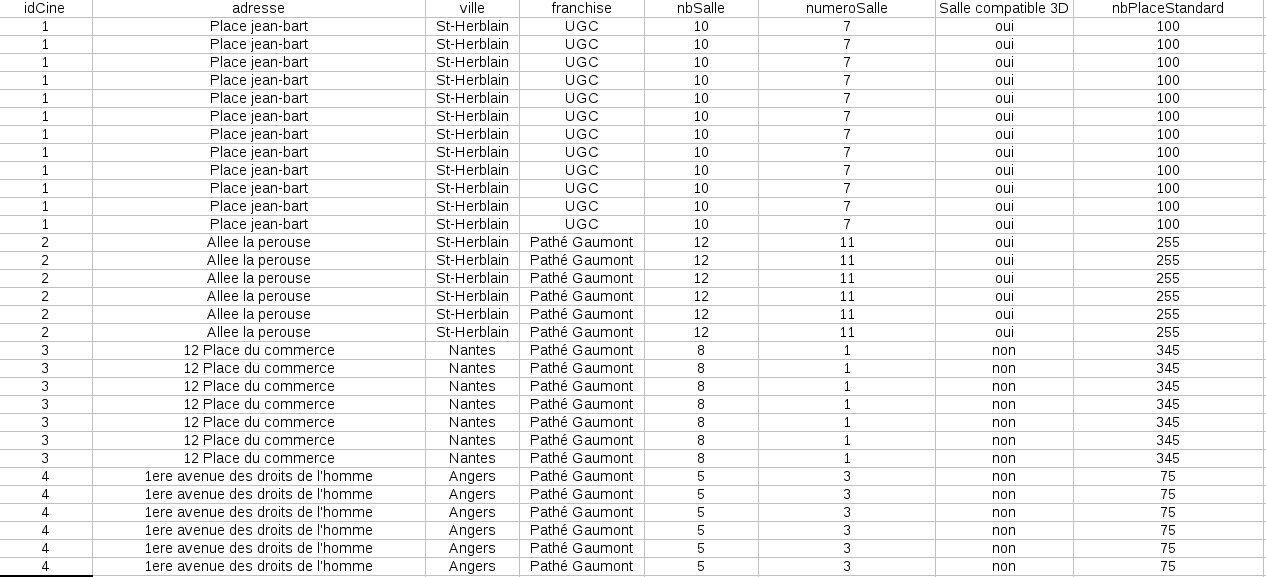
\includegraphics[height=8cm]{picture/table_p1_rogne.png}}
			\caption{Première partie de notre table contenant tous les attributs et quelques tuples}
			\label{table_p1}	
		\end{figure}			

		\begin{figure}[!h]
			\centering						
			\rotatebox{90}{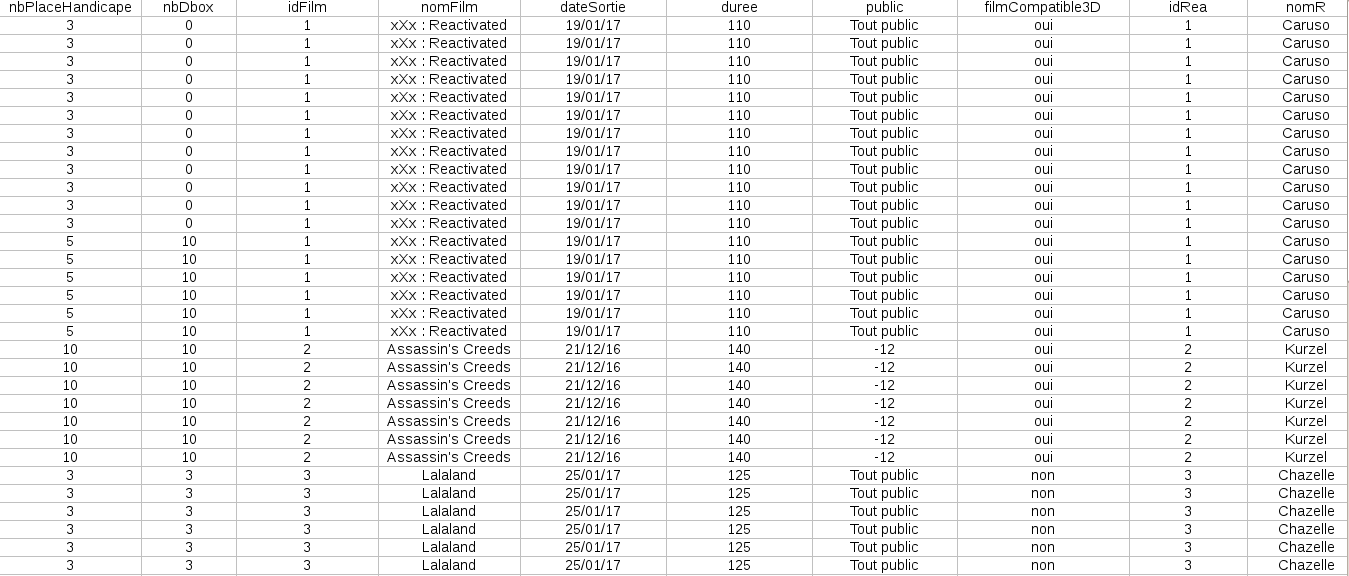
\includegraphics[height=8cm]{picture/table_p2_rogne.png}}
			\caption{Deuxième partie de notre table contenant tous les attributs et quelques tuples}
			\label{table_p2}	
		\end{figure}			

		\begin{figure}[!h]
			\centering						
			\rotatebox{90}{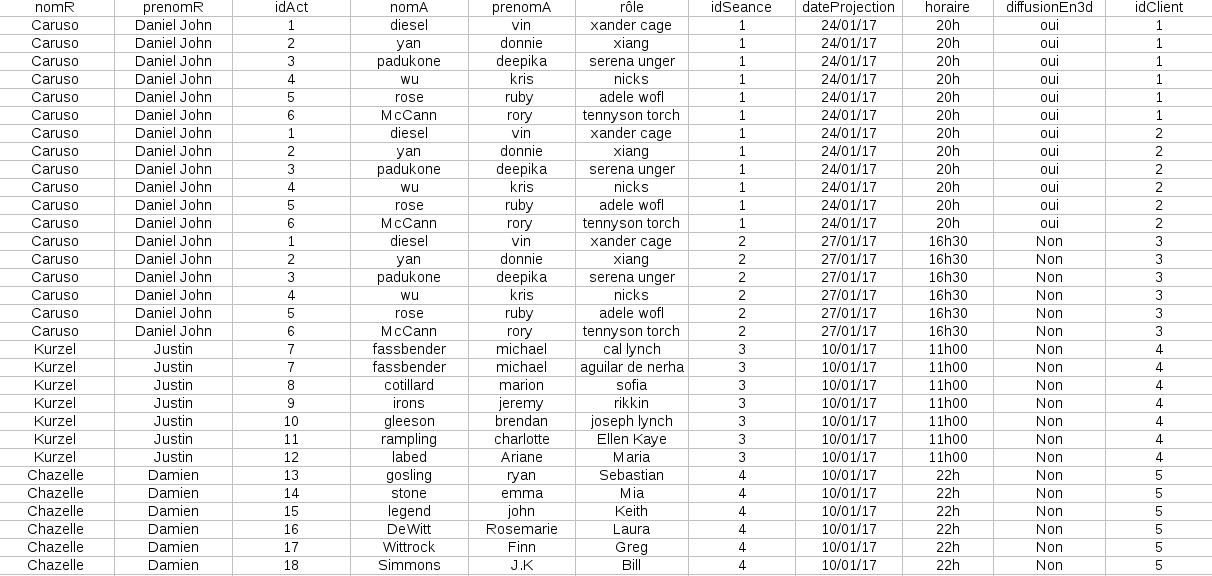
\includegraphics[height=9cm]{picture/table_p3_rogne.png}}
			\caption{Troisième partie de notre table contenant tous les attributs et quelques tuples}
			\label{table_p3}	
		\end{figure}	

		\begin{figure}[!h]
			\centering						
			\rotatebox{90}{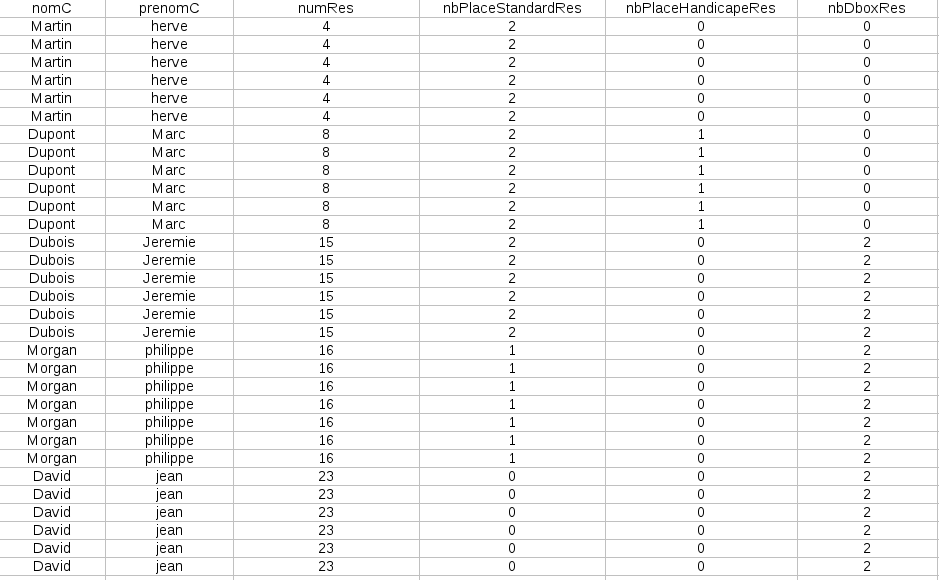
\includegraphics[height=10cm]{picture/table_p4_rogne.png}}
			\caption{Quatrième partie de notre table contenant tous les attributs et quelques tuples}
			\label{table_p4}	
		\end{figure}
		
		\begin{figure}[!h]
			\centering						
			\rotatebox{90}{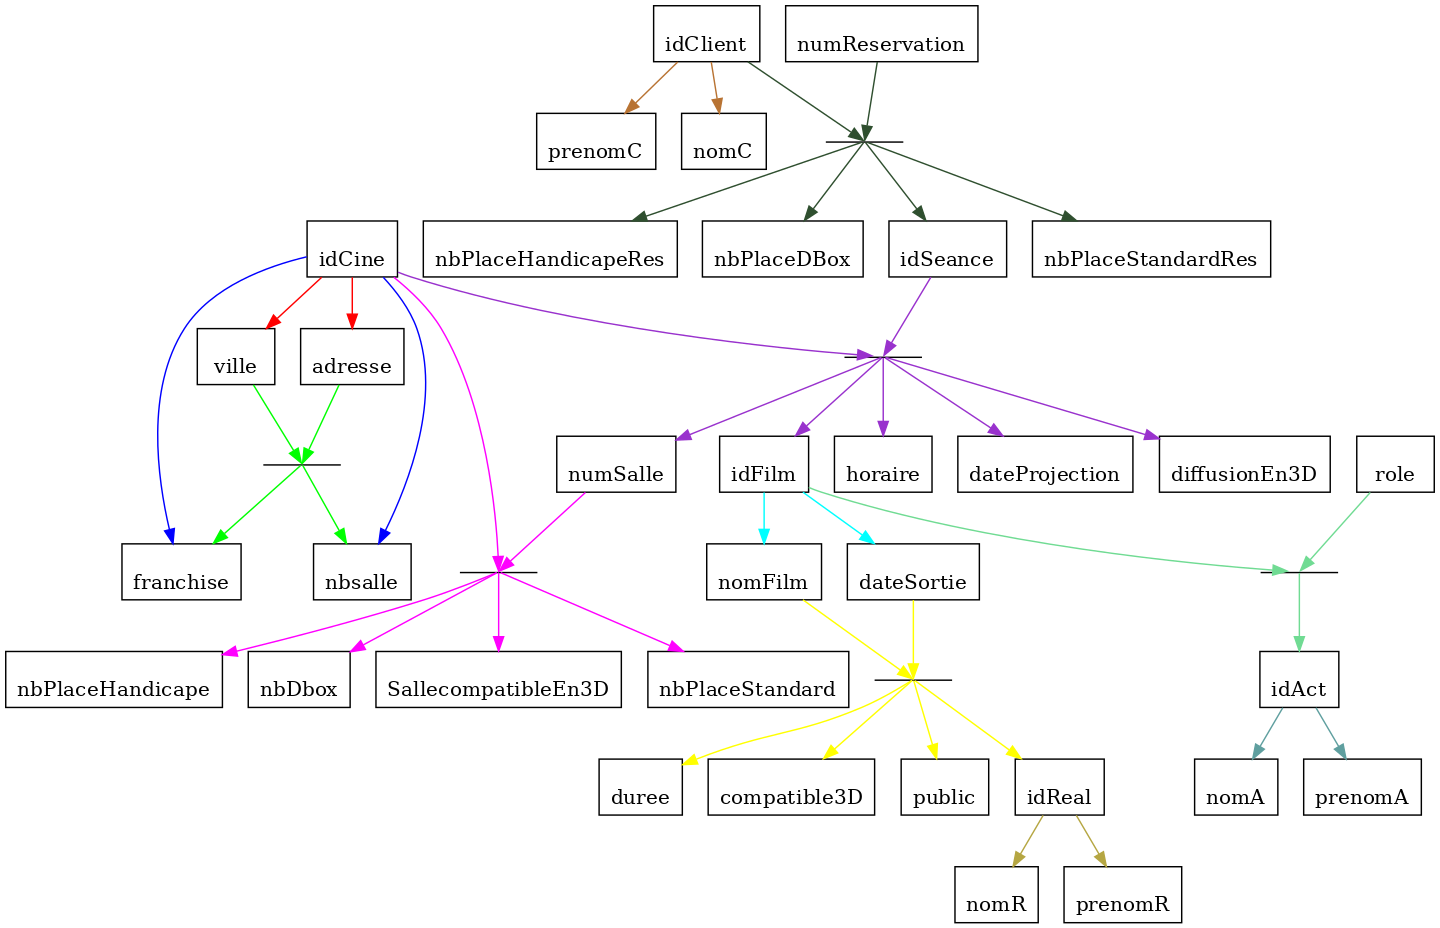
\includegraphics[height=12cm]{picture/graphe_dependances.png}}
			\caption{Graphe des dépendances}
			\label{graphe_dependances}	
		\end{figure}	
					
\end{document}
